% Created by tikzDevice version 0.12.3 on 2019-08-18 20:45:55
% !TEX encoding = UTF-8 Unicode
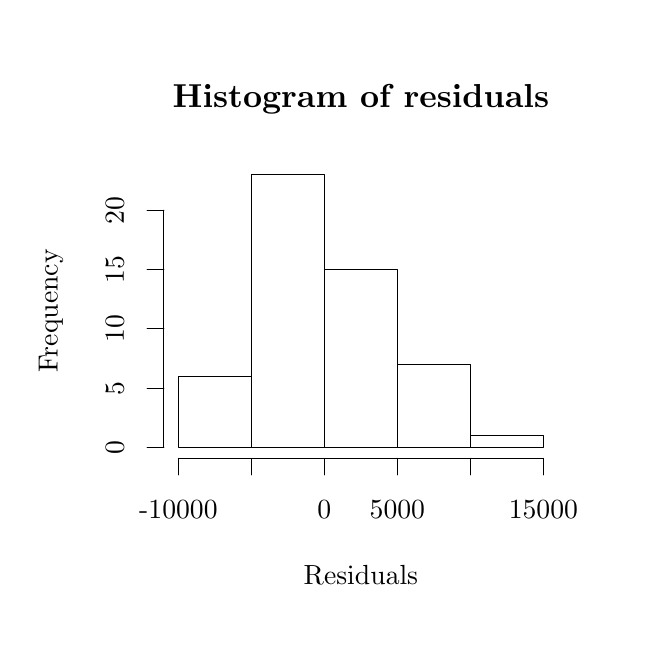
\begin{tikzpicture}[x=1pt,y=1pt]
\definecolor{fillColor}{RGB}{255,255,255}
\path[use as bounding box,fill=fillColor,fill opacity=0.00] (0,0) rectangle (216.81,216.81);
\begin{scope}
\path[clip] (  0.00,  0.00) rectangle (216.81,216.81);
\definecolor{drawColor}{RGB}{0,0,0}

\node[text=drawColor,anchor=base,inner sep=0pt, outer sep=0pt, scale=  1.20] at (120.41,188.07) {\bfseries Histogram of residuals};

\node[text=drawColor,anchor=base,inner sep=0pt, outer sep=0pt, scale=  1.00] at (120.41, 15.60) {Residuals};

\node[text=drawColor,rotate= 90.00,anchor=base,inner sep=0pt, outer sep=0pt, scale=  1.00] at ( 10.80,114.41) {Frequency};
\end{scope}
\begin{scope}
\path[clip] (  0.00,  0.00) rectangle (216.81,216.81);
\definecolor{drawColor}{RGB}{0,0,0}

\path[draw=drawColor,line width= 0.4pt,line join=round,line cap=round] ( 54.47, 61.20) -- (186.34, 61.20);

\path[draw=drawColor,line width= 0.4pt,line join=round,line cap=round] ( 54.47, 61.20) -- ( 54.47, 55.20);

\path[draw=drawColor,line width= 0.4pt,line join=round,line cap=round] ( 80.85, 61.20) -- ( 80.85, 55.20);

\path[draw=drawColor,line width= 0.4pt,line join=round,line cap=round] (107.22, 61.20) -- (107.22, 55.20);

\path[draw=drawColor,line width= 0.4pt,line join=round,line cap=round] (133.59, 61.20) -- (133.59, 55.20);

\path[draw=drawColor,line width= 0.4pt,line join=round,line cap=round] (159.96, 61.20) -- (159.96, 55.20);

\path[draw=drawColor,line width= 0.4pt,line join=round,line cap=round] (186.34, 61.20) -- (186.34, 55.20);

\node[text=drawColor,anchor=base,inner sep=0pt, outer sep=0pt, scale=  1.00] at ( 54.47, 39.60) {-10000};

\node[text=drawColor,anchor=base,inner sep=0pt, outer sep=0pt, scale=  1.00] at (107.22, 39.60) {0};

\node[text=drawColor,anchor=base,inner sep=0pt, outer sep=0pt, scale=  1.00] at (133.59, 39.60) {5000};

\node[text=drawColor,anchor=base,inner sep=0pt, outer sep=0pt, scale=  1.00] at (186.34, 39.60) {15000};

\path[draw=drawColor,line width= 0.4pt,line join=round,line cap=round] ( 49.20, 65.14) -- ( 49.20,150.82);

\path[draw=drawColor,line width= 0.4pt,line join=round,line cap=round] ( 49.20, 65.14) -- ( 43.20, 65.14);

\path[draw=drawColor,line width= 0.4pt,line join=round,line cap=round] ( 49.20, 86.56) -- ( 43.20, 86.56);

\path[draw=drawColor,line width= 0.4pt,line join=round,line cap=round] ( 49.20,107.98) -- ( 43.20,107.98);

\path[draw=drawColor,line width= 0.4pt,line join=round,line cap=round] ( 49.20,129.40) -- ( 43.20,129.40);

\path[draw=drawColor,line width= 0.4pt,line join=round,line cap=round] ( 49.20,150.82) -- ( 43.20,150.82);

\node[text=drawColor,rotate= 90.00,anchor=base,inner sep=0pt, outer sep=0pt, scale=  1.00] at ( 34.80, 65.14) {0};

\node[text=drawColor,rotate= 90.00,anchor=base,inner sep=0pt, outer sep=0pt, scale=  1.00] at ( 34.80, 86.56) {5};

\node[text=drawColor,rotate= 90.00,anchor=base,inner sep=0pt, outer sep=0pt, scale=  1.00] at ( 34.80,107.98) {10};

\node[text=drawColor,rotate= 90.00,anchor=base,inner sep=0pt, outer sep=0pt, scale=  1.00] at ( 34.80,129.40) {15};

\node[text=drawColor,rotate= 90.00,anchor=base,inner sep=0pt, outer sep=0pt, scale=  1.00] at ( 34.80,150.82) {20};
\end{scope}
\begin{scope}
\path[clip] ( 49.20, 61.20) rectangle (191.61,167.61);
\definecolor{drawColor}{RGB}{0,0,0}

\path[draw=drawColor,line width= 0.4pt,line join=round,line cap=round] ( 54.47, 65.14) rectangle ( 80.85, 90.84);

\path[draw=drawColor,line width= 0.4pt,line join=round,line cap=round] ( 80.85, 65.14) rectangle (107.22,163.67);

\path[draw=drawColor,line width= 0.4pt,line join=round,line cap=round] (107.22, 65.14) rectangle (133.59,129.40);

\path[draw=drawColor,line width= 0.4pt,line join=round,line cap=round] (133.59, 65.14) rectangle (159.96, 95.13);

\path[draw=drawColor,line width= 0.4pt,line join=round,line cap=round] (159.96, 65.14) rectangle (186.34, 69.42);
\end{scope}
\end{tikzpicture}
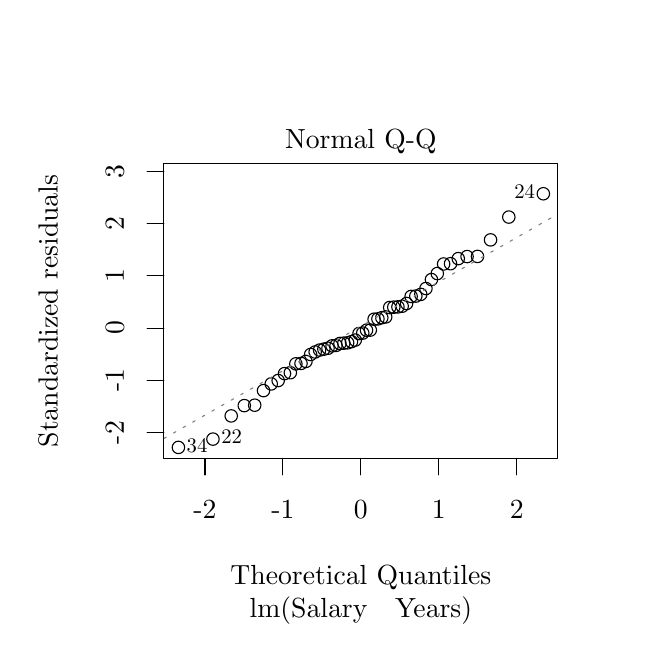
\begin{tikzpicture}[x=1pt,y=1pt]
\definecolor{fillColor}{RGB}{255,255,255}
\path[use as bounding box,fill=fillColor,fill opacity=0.00] (0,0) rectangle (216.81,216.81);
\begin{scope}
\path[clip] ( 49.20, 61.20) rectangle (191.61,167.61);
\definecolor{drawColor}{RGB}{0,0,0}

\path[draw=drawColor,line width= 0.4pt,line join=round,line cap=round] (150.30,131.42) circle (  2.25);

\path[draw=drawColor,line width= 0.4pt,line join=round,line cap=round] (173.86,148.37) circle (  2.25);

\path[draw=drawColor,line width= 0.4pt,line join=round,line cap=round] (130.82,115.69) circle (  2.25);

\path[draw=drawColor,line width= 0.4pt,line join=round,line cap=round] (112.85,102.69) circle (  2.25);

\path[draw=drawColor,line width= 0.4pt,line join=round,line cap=round] (148.01,127.96) circle (  2.25);

\path[draw=drawColor,line width= 0.4pt,line join=round,line cap=round] (142.04,120.43) circle (  2.25);

\path[draw=drawColor,line width= 0.4pt,line join=round,line cap=round] ( 85.22, 85.66) circle (  2.25);

\path[draw=drawColor,line width= 0.4pt,line join=round,line cap=round] (167.26,140.13) circle (  2.25);

\path[draw=drawColor,line width= 0.4pt,line join=round,line cap=round] (140.26,119.83) circle (  2.25);

\path[draw=drawColor,line width= 0.4pt,line join=round,line cap=round] (143.91,122.55) circle (  2.25);

\path[draw=drawColor,line width= 0.4pt,line join=round,line cap=round] (129.38,112.28) circle (  2.25);

\path[draw=drawColor,line width= 0.4pt,line join=round,line cap=round] (122.44,107.50) circle (  2.25);

\path[draw=drawColor,line width= 0.4pt,line join=round,line cap=round] (145.90,125.79) circle (  2.25);

\path[draw=drawColor,line width= 0.4pt,line join=round,line cap=round] ( 90.51, 89.30) circle (  2.25);

\path[draw=drawColor,line width= 0.4pt,line join=round,line cap=round] (117.00,103.35) circle (  2.25);

\path[draw=drawColor,line width= 0.4pt,line join=round,line cap=round] (158.77,134.10) circle (  2.25);

\path[draw=drawColor,line width= 0.4pt,line join=round,line cap=round] (155.59,133.35) circle (  2.25);

\path[draw=drawColor,line width= 0.4pt,line join=round,line cap=round] (133.79,115.91) circle (  2.25);

\path[draw=drawColor,line width= 0.4pt,line join=round,line cap=round] (119.73,106.29) circle (  2.25);

\path[draw=drawColor,line width= 0.4pt,line join=round,line cap=round] (114.25,102.82) circle (  2.25);

\path[draw=drawColor,line width= 0.4pt,line join=round,line cap=round] ( 73.55, 76.52) circle (  2.25);

\path[draw=drawColor,line width= 0.4pt,line join=round,line cap=round] ( 66.95, 68.14) circle (  2.25);

\path[draw=drawColor,line width= 0.4pt,line join=round,line cap=round] (152.80,131.52) circle (  2.25);

\path[draw=drawColor,line width= 0.4pt,line join=round,line cap=round] (186.34,156.79) circle (  2.25);

\path[draw=drawColor,line width= 0.4pt,line join=round,line cap=round] (138.56,119.69) circle (  2.25);

\path[draw=drawColor,line width= 0.4pt,line join=round,line cap=round] (127.96,112.00) circle (  2.25);

\path[draw=drawColor,line width= 0.4pt,line join=round,line cap=round] (135.33,116.16) circle (  2.25);

\path[draw=drawColor,line width= 0.4pt,line join=round,line cap=round] (132.29,115.81) circle (  2.25);

\path[draw=drawColor,line width= 0.4pt,line join=round,line cap=round] (162.54,134.15) circle (  2.25);

\path[draw=drawColor,line width= 0.4pt,line join=round,line cap=round] (121.08,106.45) circle (  2.25);

\path[draw=drawColor,line width= 0.4pt,line join=round,line cap=round] (107.02,100.64) circle (  2.25);

\path[draw=drawColor,line width= 0.4pt,line join=round,line cap=round] ( 82.04, 80.39) circle (  2.25);

\path[draw=drawColor,line width= 0.4pt,line join=round,line cap=round] (125.18,111.46) circle (  2.25);

\path[draw=drawColor,line width= 0.4pt,line join=round,line cap=round] ( 54.47, 65.14) circle (  2.25);

\path[draw=drawColor,line width= 0.4pt,line join=round,line cap=round] ( 78.27, 80.24) circle (  2.25);

\path[draw=drawColor,line width= 0.4pt,line join=round,line cap=round] (123.81,107.53) circle (  2.25);

\path[draw=drawColor,line width= 0.4pt,line join=round,line cap=round] ( 88.01, 88.08) circle (  2.25);

\path[draw=drawColor,line width= 0.4pt,line join=round,line cap=round] (103.89, 99.62) circle (  2.25);

\path[draw=drawColor,line width= 0.4pt,line join=round,line cap=round] (100.55, 96.21) circle (  2.25);

\path[draw=drawColor,line width= 0.4pt,line join=round,line cap=round] (109.99,101.84) circle (  2.25);

\path[draw=drawColor,line width= 0.4pt,line join=round,line cap=round] (118.37,103.92) circle (  2.25);

\path[draw=drawColor,line width= 0.4pt,line join=round,line cap=round] ( 92.80, 91.80) circle (  2.25);

\path[draw=drawColor,line width= 0.4pt,line join=round,line cap=round] (126.56,111.58) circle (  2.25);

\path[draw=drawColor,line width= 0.4pt,line join=round,line cap=round] (111.43,102.00) circle (  2.25);

\path[draw=drawColor,line width= 0.4pt,line join=round,line cap=round] (102.25, 98.71) circle (  2.25);

\path[draw=drawColor,line width= 0.4pt,line join=round,line cap=round] (105.48,100.31) circle (  2.25);

\path[draw=drawColor,line width= 0.4pt,line join=round,line cap=round] ( 94.91, 92.13) circle (  2.25);

\path[draw=drawColor,line width= 0.4pt,line join=round,line cap=round] ( 96.90, 95.33) circle (  2.25);

\path[draw=drawColor,line width= 0.4pt,line join=round,line cap=round] (108.52,100.97) circle (  2.25);

\path[draw=drawColor,line width= 0.4pt,line join=round,line cap=round] (115.63,102.93) circle (  2.25);

\path[draw=drawColor,line width= 0.4pt,line join=round,line cap=round] ( 98.77, 95.48) circle (  2.25);

\path[draw=drawColor,line width= 0.4pt,line join=round,line cap=round] (136.92,117.14) circle (  2.25);
\end{scope}
\begin{scope}
\path[clip] (  0.00,  0.00) rectangle (216.81,216.81);
\definecolor{drawColor}{RGB}{0,0,0}

\path[draw=drawColor,line width= 0.4pt,line join=round,line cap=round] ( 64.08, 61.20) -- (176.73, 61.20);

\path[draw=drawColor,line width= 0.4pt,line join=round,line cap=round] ( 64.08, 61.20) -- ( 64.08, 55.20);

\path[draw=drawColor,line width= 0.4pt,line join=round,line cap=round] ( 92.24, 61.20) -- ( 92.24, 55.20);

\path[draw=drawColor,line width= 0.4pt,line join=round,line cap=round] (120.40, 61.20) -- (120.40, 55.20);

\path[draw=drawColor,line width= 0.4pt,line join=round,line cap=round] (148.57, 61.20) -- (148.57, 55.20);

\path[draw=drawColor,line width= 0.4pt,line join=round,line cap=round] (176.73, 61.20) -- (176.73, 55.20);

\node[text=drawColor,anchor=base,inner sep=0pt, outer sep=0pt, scale=  1.00] at ( 64.08, 39.60) {-2};

\node[text=drawColor,anchor=base,inner sep=0pt, outer sep=0pt, scale=  1.00] at ( 92.24, 39.60) {-1};

\node[text=drawColor,anchor=base,inner sep=0pt, outer sep=0pt, scale=  1.00] at (120.40, 39.60) {0};

\node[text=drawColor,anchor=base,inner sep=0pt, outer sep=0pt, scale=  1.00] at (148.57, 39.60) {1};

\node[text=drawColor,anchor=base,inner sep=0pt, outer sep=0pt, scale=  1.00] at (176.73, 39.60) {2};

\path[draw=drawColor,line width= 0.4pt,line join=round,line cap=round] ( 49.20, 70.52) -- ( 49.20,164.87);

\path[draw=drawColor,line width= 0.4pt,line join=round,line cap=round] ( 49.20, 70.52) -- ( 43.20, 70.52);

\path[draw=drawColor,line width= 0.4pt,line join=round,line cap=round] ( 49.20, 89.39) -- ( 43.20, 89.39);

\path[draw=drawColor,line width= 0.4pt,line join=round,line cap=round] ( 49.20,108.26) -- ( 43.20,108.26);

\path[draw=drawColor,line width= 0.4pt,line join=round,line cap=round] ( 49.20,127.13) -- ( 43.20,127.13);

\path[draw=drawColor,line width= 0.4pt,line join=round,line cap=round] ( 49.20,146.00) -- ( 43.20,146.00);

\path[draw=drawColor,line width= 0.4pt,line join=round,line cap=round] ( 49.20,164.87) -- ( 43.20,164.87);

\node[text=drawColor,rotate= 90.00,anchor=base,inner sep=0pt, outer sep=0pt, scale=  1.00] at ( 34.80, 70.52) {-2};

\node[text=drawColor,rotate= 90.00,anchor=base,inner sep=0pt, outer sep=0pt, scale=  1.00] at ( 34.80, 89.39) {-1};

\node[text=drawColor,rotate= 90.00,anchor=base,inner sep=0pt, outer sep=0pt, scale=  1.00] at ( 34.80,108.26) {0};

\node[text=drawColor,rotate= 90.00,anchor=base,inner sep=0pt, outer sep=0pt, scale=  1.00] at ( 34.80,127.13) {1};

\node[text=drawColor,rotate= 90.00,anchor=base,inner sep=0pt, outer sep=0pt, scale=  1.00] at ( 34.80,146.00) {2};

\node[text=drawColor,rotate= 90.00,anchor=base,inner sep=0pt, outer sep=0pt, scale=  1.00] at ( 34.80,164.87) {3};

\path[draw=drawColor,line width= 0.4pt,line join=round,line cap=round] ( 49.20, 61.20) --
	(191.61, 61.20) --
	(191.61,167.61) --
	( 49.20,167.61) --
	( 49.20, 61.20);
\end{scope}
\begin{scope}
\path[clip] (  0.00,  0.00) rectangle (216.81,216.81);
\definecolor{drawColor}{RGB}{0,0,0}

\node[text=drawColor,anchor=base,inner sep=0pt, outer sep=0pt, scale=  1.00] at (120.41, 15.60) {Theoretical Quantiles};

\node[text=drawColor,rotate= 90.00,anchor=base,inner sep=0pt, outer sep=0pt, scale=  1.00] at ( 10.80,114.41) {Standardized residuals};
\end{scope}
\begin{scope}
\path[clip] ( 49.20, 61.20) rectangle (191.61,167.61);
\definecolor{drawColor}{gray}{0.50}

\path[draw=drawColor,line width= 0.4pt,dash pattern=on 1pt off 3pt ,line join=round,line cap=round] ( 49.20, 68.34) -- (191.61,149.47);
\end{scope}
\begin{scope}
\path[clip] (  0.00,  0.00) rectangle (216.81,216.81);
\definecolor{drawColor}{RGB}{0,0,0}

\node[text=drawColor,anchor=base,inner sep=0pt, outer sep=0pt, scale=  1.00] at (120.41,  3.60) {lm(Salary ~ Years)};
\end{scope}
\begin{scope}
\path[clip] (  0.00,  0.00) rectangle (216.81,216.81);
\definecolor{drawColor}{RGB}{0,0,0}

\node[text=drawColor,anchor=base,inner sep=0pt, outer sep=0pt, scale=  1.00] at (120.41,173.01) {Normal Q-Q};
\end{scope}
\begin{scope}
\path[clip] (  0.00,  0.00) rectangle (216.81,216.81);
\definecolor{drawColor}{RGB}{0,0,0}

\node[text=drawColor,anchor=base east,inner sep=0pt, outer sep=0pt, scale=  0.75] at (183.34,155.07) {24};

\node[text=drawColor,anchor=base west,inner sep=0pt, outer sep=0pt, scale=  0.75] at ( 57.47, 63.42) {34};

\node[text=drawColor,anchor=base west,inner sep=0pt, outer sep=0pt, scale=  0.75] at ( 69.95, 66.41) {22};
\end{scope}
\end{tikzpicture}
